\subsubsection{Clock Konfiguration}
\label{sec:CubeMXClock}

Der STM32F412 hat einen $f_{HSE}=8.000\si{MHz}$ Clock von einem Quarz Oszillator.
Dazu muss unter \texttt{System Core > RCC} die High Speed Clock (HSE) auf \texttt{Crystal/Ceramic Resonator} gesetzt werden. Die Abbildung \ref{pic:CubeMX_RCC} zeigt die notwendigen Einstellungen.

Da der TLV320 im Master Mode betrieben wird, kommt auch der Clock für die I\textsuperscript{2}S Peripherie vom TLV320 über den \texttt{CLK\_OUT} Pin.
Die I\textsuperscript{2}S Clock Frequenz beträgt $f_{clk}=12.288\si{MHz}$.
Im \texttt{RCC} Reiter muss die Audio Clock Input (\texttt{I2S\_CKIN}) aktiviert werden.

\begin{figure}[H]
	\centering
	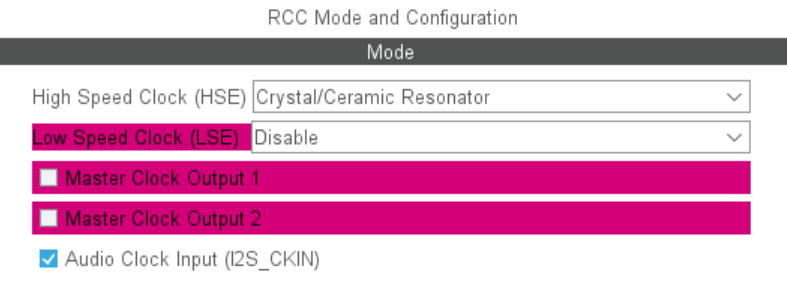
\includegraphics[width=0.6\linewidth]{CubeMX_RCC}
	\caption{Auswahl der externen Clock (HSE)}
	\label{pic:CubeMX_RCC}
\end{figure}

Die maximale Taktfrequenz des STM32F412 liegt bei $f_{CPU}=100\si{MHz}$.
Damit die Geschwindigkeit erreicht wird, wird der interne PLL so konfiguriert, dass die CPU die maximale Taktfrequenz zugewiesen bekommt. Die Abbildung \ref{pic:CubeMX_Clock} zeigt alle notwendigen Konfigurationen inklusive der externen I\textsuperscript{2}S Clock.

\begin{figure}[H]
	\centering
	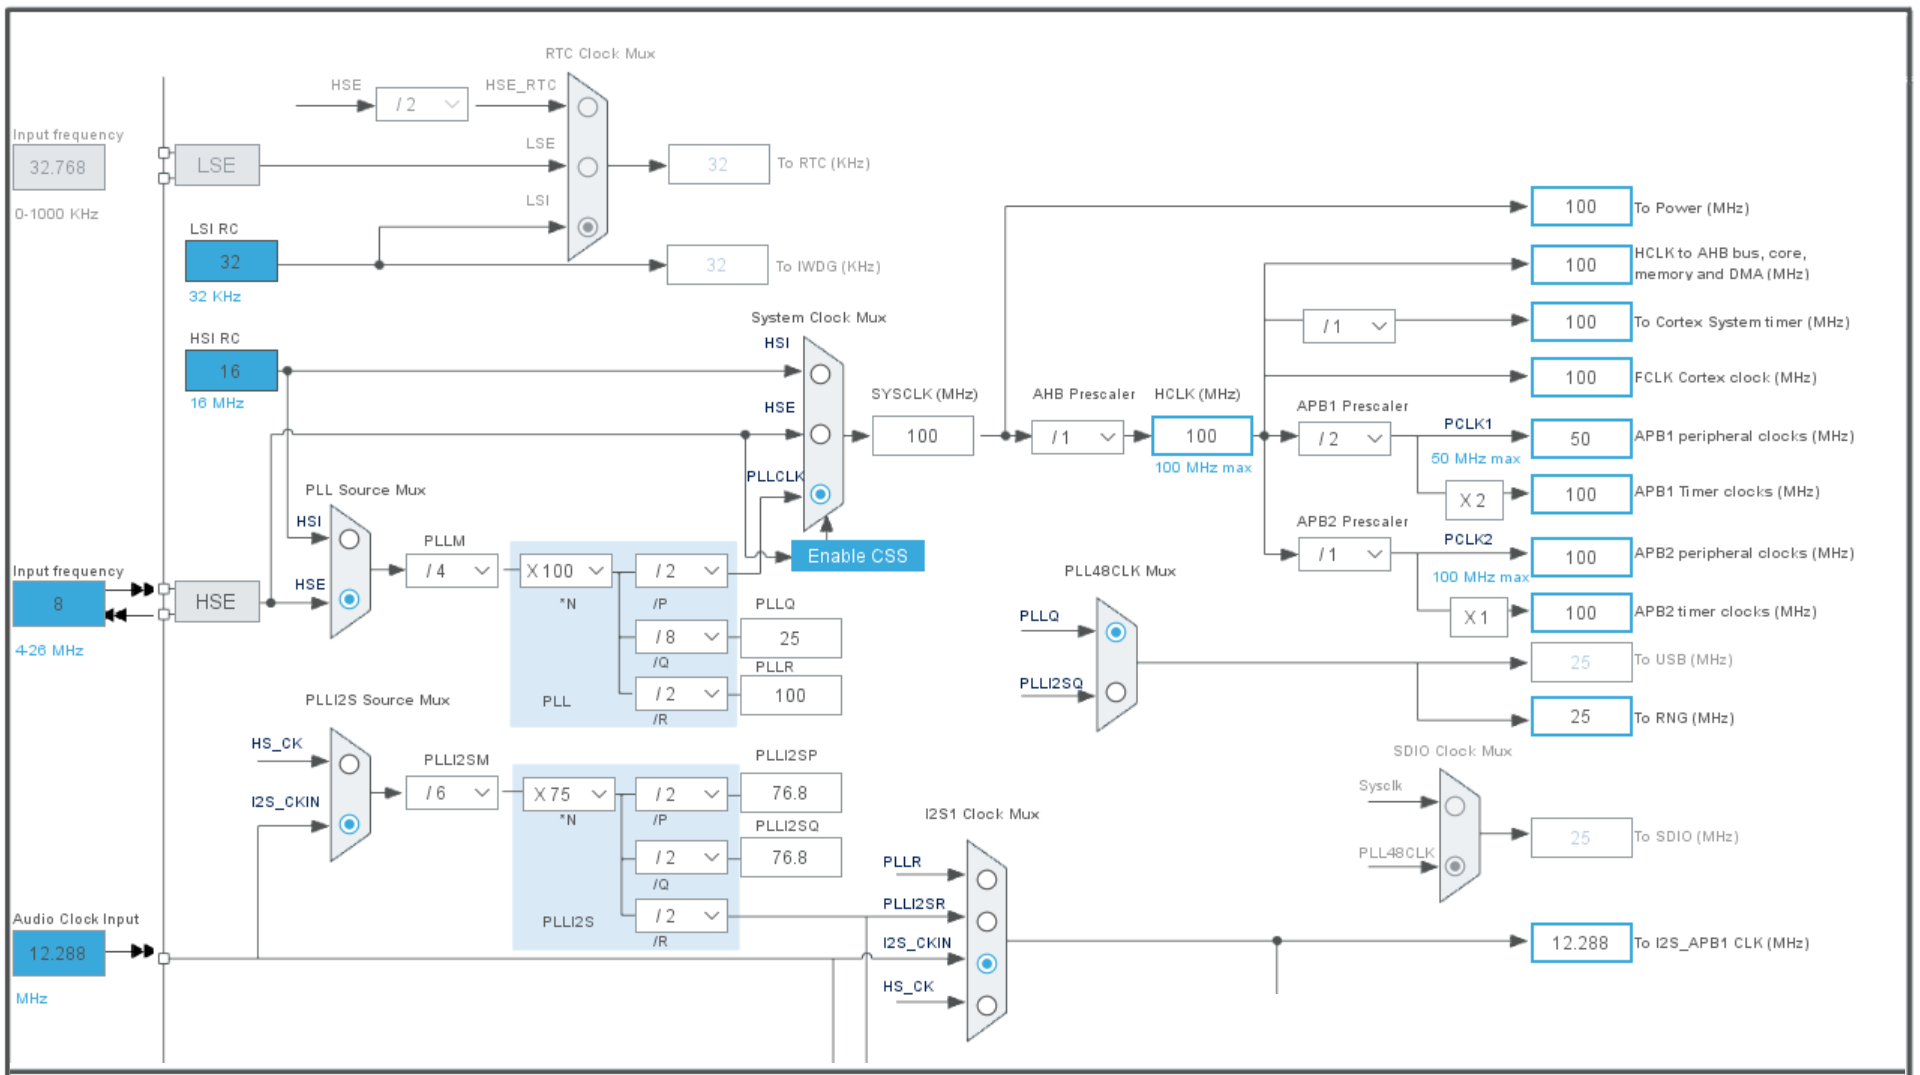
\includegraphics[width=1.0\linewidth]{CubeMX_Clock}
	\caption{Gesamtübersicht der Clockkonfiguration mit $f_{CPU}=100\si{MHz}$}
	\label{pic:CubeMX_Clock}
\end{figure}

